\documentclass[10pt,a4paper]{article}
% for importing matlab codes
\usepackage[numbered]{mcode}
% for margining standards
\usepackage[left=3cm,right=3cm,top=3cm,bottom=3cm]{geometry}
% for counting references as a section
\usepackage[numbib,notlof,notlot,nottoc]{tocbibind}
% useful packages
\usepackage{
                graphicx, setspace, fontspec, caption,
                subcaption, float, polyglossia, rotating,
                lscape, pdflscape, indentfirst, tocloft
            }
% paragraph related package
\usepackage[parfill]{parskip}
% use bzar font(THIS MUST BE LOADED BEFORE XePerian PACKAGE)
\setmainfont{BZar.ttf}
% the dear XePersian package
\usepackage{xepersian}
%
% General settings goes here.
%
% lines space
\renewcommand{\baselinestretch}{1.5}
% paragraph first line indention
\setlength{\parindent}{1cm}
% paragraph spacing
\setlength{\parskip}{1em}
% set graphics' path
\graphicspath{ {images/} }
% make table of content dotted
\renewcommand{\cftsecleader}{\cftdotfill{\cftdotsep}}
%
% DOCUMENT BEGIN
%
\begin{document}
\title{استفاده از متد رگراسیون لاجیستیک برای طبقه بندی عکس های پزشکی با استفاده از سیگنال \lr{CXR}}
\author{داریوش حسن پور آده}
\date{۹۳۰۸۱۶۴}
\maketitle
\null
\vfill
\newpage
\section{مقدمه}
پردازش تصاویر امروزه بیشتر به موضوع پردازش تصویر دیجیتال گفته می‌شود که شاخه‌ای از دانش رایانه است که با پردازش سیگنال دیجیتال که نماینده تصاویر برداشته شده با دوربین دیجیتال یا پویش شده توسط پویشگر هستند سر و کار دارد. تصاویربرداری پزشکی به تکنیک و فرایند مورد استفاده برای ساختن تصاویری از بدن انسان (یا بخش‌ها و عملکردهای آن) برای اهداف کلینیکی (روش‌های پزشکی که در جستجوی شناخت، درمان و بررسی بیماری‌ها هستند.) یا علوم پزشکی (شامل مطالعات آناتومیک و فیزیولوژیک) است. تصویربرداری پزشکی، تداخلی از چند شاخه علوم همانند فیزیک 
پزشکی، مهندسی پزشکی، زیست‌شناسی، و اپتیک می‌باشد.
باتوجه به رشد روز افزون تکنولوژی‌های علوم کامپیوتر و تصویربرداری پزشکی امروزه بیش‌ از‌ پیش جامعه ی پزشکی نیازمند به سیستم های خبره برای بررسی تصاویر پزشکی برای مسایل تحلیلی و آنالیزی هست؛ بنابراین دسته بندی و تحلیل تصاویر پزشکی یکی از به روزترین مسایل مطرح در این زمینه میباشد.
\tableofcontents
\newpage
\section{معرفی روش \lr{CXR}}
در سال
\date{1370}
آقای تانگ و همکارانش
\cite{RP}
 اولین روش تبدیل الگوی ۲ بعدی به ۱ بعدی با نام \تاکید{تصویر حلقه\زیرنویس{
\lr{Ring Projection}
}} را ارائه داد.
که این تبدیل الگوی دوبعدی را به الگوی تک بعدی با استفاده از تصویر کردن الگوهای روی دایره هایی با شعاع های متفاوت تبدیل می کند.
در سال \تاریخ{۱۳۷۸} آقای تاوء و همکارانش
\cite{CP}
 روش دیگری را با نام \تاکید{تصویر مرکزی\زیرنویس{
\lr{Central Projection}
}} 
ارائه دادند که همانند تصویر حلقه  الگوی ۲ بعدی به ۱ بعدی تبدیل میکرد با این تفاوت که الگوهایی که با زاویه ی متفاوت از یک دیگر قرار داشتند به نقاط متفاوتی تصویر می کرد.\بند
هر دوی روش های تصویر حقله و تصویر مرکزی یک الگوی دو بعدی را به یک بعد تبدیل میکنند با این تفاوت که هر کدام از آن ها از دیدگاه تفاوتی به الگو نگاه کرده و تبدیلاتشان را از دیدگاه متفاوتی اعمال میکنند.
در این اواخر آقای تانگ و همکارانش 
\cite{WRP, FRP}
کاربردهای دیگری از روش تصویر حلقه ارائه دادند که خارج از حوضه ی این نوشتار می باشند.\بند
با توجه به اینکه روش تصویر مرکزی اطلاعات روی خطوط با زاویه های متفاوت را نمی تواند استخراج کند و از سمت دیگر روش تصویر حلقه اطلاعات رو شعاع های متفاوت را نمی تواند استخراج کنند هردوی این روش ها دارای از دست رفتگی داده ای می باشند. روش
\lr{CXR}\زیرنویس{ابداع اینجانب در پروژه ی مقطع کارشناسی میباشد.}
با ترکیب این دو روش توانست یک تبدیل بهینه ای بدست آورد که مشکل از دست رفتگی داده ها در روش های قبلی را ندارد؛ روش
\lr{CXR}
تمامی خواص روش های والدش را دارد بنابراین خواص معرفی شده در روش های تصویر حلقوی و مرکزی در این روش نیز صادق اند. بحث راجع به روش
\lr{CXR}
خارج از حوضه ی این نوشتار می باشد.\بند
ماهیت همگی روش های معرفی شده در بالا یک سیگنال یک بعدی بوده و در شکل های زیر نمونه هایی از عکس ها و سیگنال های
\lr{CXR}
مربوط به آن عکس ها آورده شده است.(جهت داشتن دید بهتر راجع به داده هایی که برای یادگیری استفاده خواهیم کرد.)

\begin{figure}[H]
    \centering
    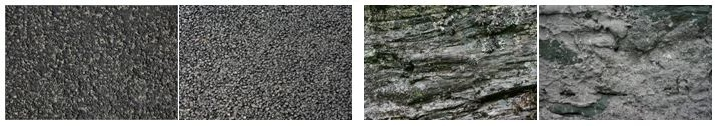
\includegraphics[width=1\textwidth]{txt-1}
    \caption{تعدادی بافت از ۲ گونه متفاوت}
    \label{fig:حروف}
\end{figure}
\begin{figure}[H]
    \centering
    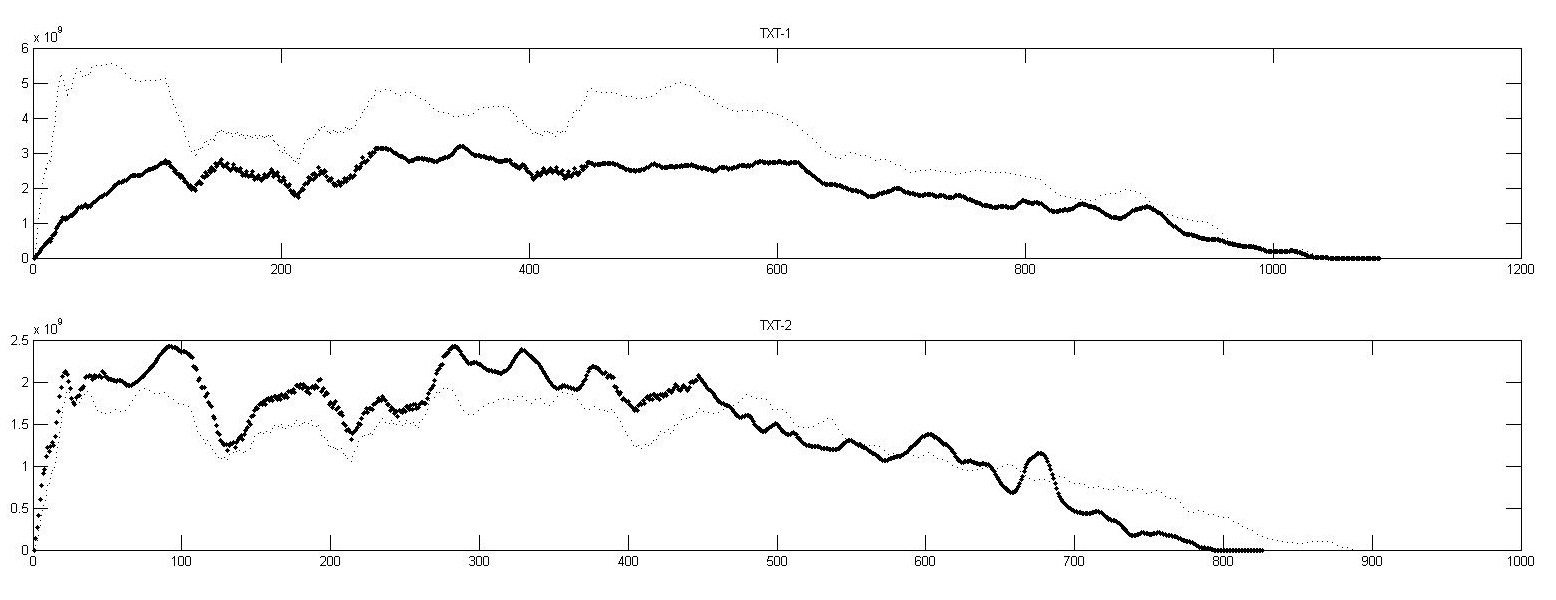
\includegraphics[width=1\textwidth]{txt-2}
    \caption{سیگناهای
\lr{CXR}
متناظر با بافت های شکل
\ref{fig:حروف}
    }
    \label{fig:سیگنال-حروف}
\end{figure}

همانطور که در شکل های
\ref{fig:حروف}
و
\ref{fig:سیگنال-حروف}
مشاهده میشود بافت های مشابه دارای سیگنالهای مشابه هستند که ما در این پروژه میخواهیم که از این ویژگی سیگنال ها برای طبقه بندی عکس های پزشکی استفاده کنیم.

\section{مجموعه داده های ورودی}
از آنجایی که موضوع پروژه طبقه بندی عکس ها می­باشد, نیاز به داده­های تصویری وجود دارد. در مورد جمع آوری داده؛ بدیهی است که نیاز به تصاویر ام.ار.ای وجود دارد به باتوجه به زیرساخت ضعیف موجود در نظام پزشکی ایران در مستندسازی اطلاعات پزشکی دسترسی به دیتاست مرغوب تصاویر ام.ار.ای یا امکان نیست و یا نیاز به داشتن مجوز از سازمان های مرتبط هست که در زمان انجام پروژه های کارشناسی امکان این امر محیا نشد برای این منظور ما 21 عدد عکس از 5 اندام مذکور را توسط موتور جستجوی گوگل استخراج کردیم و هر کدام از عکس ها با درجات ۰-۹۰-۱۸۰-۲۷۰ درجه دوران و 3 سایز متفاوت علاوه بر سایز اصلی عکس شامل سایز های {128*128 - 256*256 - 512*512} چندبرابر شده اند.
مجموعه ی داده ی ورودی به برنامه ی طبقه بندی کننده برداری از ویژگی سیگنال(
\lr{CXR} - 
همانند سیگنال های شکل\ref{fig:سیگنال-حروف}
) استخراج شده از تصاویر MRI گرفته شده از 5 ناحیه بدن که شامل ناحیه های کل بدن, مغز, زانو, شانه و ستون فقرات میباشد. که ویژگی های مورد استفاده شامل در واقع مقادیر سیگنال بوده اند.
\subsection{پیش پردازش}
همانطور که در شکل
\ref{fig:سیگنال-حروف}
می بینیم تعداد اندیس های سیگنال برای استفاده به عنوان بردار ویژگی بسیار زیاد بوده است و بدیهی است که این ویژگی ها دارای ارتباط خطی با یکی دیگر نیستند و در صورتی که بخوام ارتباط های غیر خطی این ویژکی ها را در یاگیری طبقه بندمان در نظر بگیریم حجم ویژگی های توانی بیشتر خواهد شد. بنابراین پیش پردازش های جهت کاهش تعداد ویژگی ها(حذف ویژگی های غیر ضروری) و افزایش دقت طبقه بند در ۳ مرحله انجام گرفته است. که در قسمت های زیر آمده اند.
\subsubsection{هنگام بارگذاری عکس ها}
در طبقه بندی عکس های پزشکی عکس ها با اندازه کوچک میتواند نماینده خوبی از داده های عکس اصلی باشد برای همین هنگام بارگذاری عکس ها و قبل از استخراج ویژگی های سیگنال
\lr{CXR}
تمامی عکس ها به اندازه ۶۴
$\times$
۶۴ پیکسل تغییر اندازه داده می شوند.
\subsubsection{بعد از استخراج سیگنال \lr{CXR}}
با اینکه تغییر اندازه عکس ها در کاهش تعداد مقادیر سیگنال
\lr{CXR}
موثر واقع شد ولی کماکان از نظر محاسباتی زیاد میباشند(با توجه به اینکه بعدها ویژگی های ارتباطات غیر خطی ویژگی های اصلی به ویژگی های اصلی نیز اضافه خواهند شد.) بعد از استخراج سیگنال
\lr{CXR}
میانگین هر ۱۰ ویژگی به عنوان یک ویژگی در نظر گرفته میشود.
\subsubsection{ایجاد ویژگی های ارتباط غیرخطی ویژگی های اصلی}
همانطور که از شکل
\ref{fig:سیگنال-حروف}
می بینیم ویژگی ها حتما باید دارای ارتباط غیرخطی با یکی دیگر باشند. برای همین منظور ویژگی های اصلی با یک درجه ای که در قسمت آزمایشات این نوشتار آمده است با هم مرتبط میشوند و به عنوان ویژگی جدید در نظر گرفته میشوند.
\section{الگوریتم رگرسیون لجستیک}
امروزه در بيشتر پژوهش‌ها در پي رسيدن به هدفي خاص با استفاده از چندين عامل ديگر هستيم بنحوي كه مقدار بهينه را بدهد. كه در آمار با روش‌هاي مختلف رگرسيوني به انجام اين چنين كارهايي پرداخته و نتايج تحليل مي‌شود.
در رگرسيون به‌وسيله متغيرهاي مستقل، متغير پاسخ  برآورد مي‌شود. كه اين متغير پاسخ همان هدف اصلي در پژوهش‌ها مي‌باشد.\بند
همانطور كه گفته شد روش‌هاي مختلف رگرسيوني با توجه به نوع عامل‌ها در تحقيقات استفاده مي‌شود. رگرسيون لجستيك نيز حالت خاصي از رگرسيون است كه در مواردي كه متغير پاسخ دو گزينه‌اي يا چند گزينه‌اي است؛ يعني فقط دو يا چند حالت متفاوت براي متغير پاسخ وجود دارد، به‌كار مي‌رود.
اين حالت بيشتر در تحقيقات پزشكي و جامعه شناسي مورد استفاده قرار مي‌گيرد. مثل عامل‌هايي كه در بيماري‌هاي سرطاني موثرند. يا در اين تحقيق مانند مرده يا زنده بودن راننده، وضعيت خودرو پس از تصادف، وضعيت جسمي راننده و ...\بند
هرگاه بخواهيم رابطه‌اي ميان مجموعه‌اي از Xها را با يك متغير وابسته مانند Y مشخص كنيم با يك مسأله چند متغيره روبرو هستيم.
 در تحليل چنين مسائلي از چندين روش رياضي استفاده مي‌شود.
رگرسيون لجستيك يك مدل رياضي است كه مي‌تواند براي توصيف رابطه چندين متغير X با يك متغير وابسته دو حالتي يا چند حالتي(متغيري كه فقط داراي دو يا چند وضعيت متفاوت است) به عنوان  Yمورد استفاده قرار گيرد.
منظور از متغير دو حالتي، متغيري است كه فقط داراي دو جواب مي‌باشد، مانند مردن يا زنده ماندن، كمربند ايمني بستن يا نبستن، حاضر بودن يا غايب بودن و بيمار بودن يا بيمار نبودن. اغلب براي اين متغير‌ها از كدهاي صفر و يك استفاده مي‌شود، كد يك را براي حالت مثبت بودن (موفقيت) آن خاصيت (بيمار بودن) و كد صفر براي منفي بودن (شكست) آن به كار مي‌رود.
تابع لاجستیک و مشتق آن به صورت زیر تعریف میشود:
\begin{figure}[H]
    \centering
    \begin{subfigure}[b]{0.49\textwidth}
        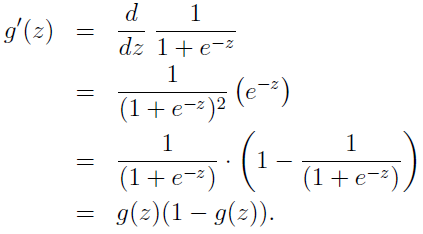
\includegraphics[width=\textwidth]{gzprim}
        \caption{تابع لاجستیک}
    \end{subfigure} 
    \begin{subfigure}[b]{0.49\textwidth}
        \begin{center}
        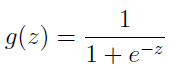
\includegraphics[scale=0.5]{gz}
        \end{center}
        \caption{مشتق تابع لاجستیک}
    \end{subfigure}
    \caption{تابع لاجستیک و مشتق آن}
    \label{fig:تابع لاجستیک}
\end{figure}
احتمال تعلق به هر دسته را میتوان بصورت تابع لجستيک در نظر گرفت:
\begin{equation}
P(Y=1 \mid X = <1, x_1,...,x_n>) = \frac{1}{1+exp(-\theta^TX)} = \frac{1}{1+exp(-(\theta_0 + \Sigma\theta_ix_i))}
\label{eq:تابع احتمال لاجستیک}
\end{equation}
که در معادله
\ref{eq:تابع احتمال لاجستیک}
$\theta_i$
ها توسط گرادیان نزولی تعیین میشوند.
\section{پیاده سازی}
در بحث پیاده سازی از آنجایی که ماهیت رگراسیون لاجستیک دودویی میباشد یعنی برای طبقه بندی ۰ یا ۱ میباشد برای طبقع بندی هریک از ۵ کلاس تعریف شده در مقدمه ی نوشتار یک آموزش لاجستیک مستقل انجام می شود و ضرایب یادگرفته شده برای آن کلاس ذخیره میشود. سپس جهت طبقه بندی/تست نمونه ی مورد نظر را به هریک از ۵ طبقه بند میدهیم و هریک که احتمال بالاتری را به عنوان نتیجه برگرداند؛ نمونه را به آن کلاس انتساب می دهیم.\بند
برای جستجو در فضای پاسخ ها از تابع
$fminunc$
متلب استفاده میکنیم که این تابع با استفاده از متدهایی(که در اینجا ما متد رگراسیون را انتخاب کرده بودیم) به دنبال کمینه محلی می گردد.\بند
الگوریتم نوشته شده برای یادگیری کلیه کلاس ها به صورت زیر است:
\begin{latin}
\lstinputlisting{../train_logistic.m}
\end{latin}
\section{ترکیب(پیچش) ویژگی های}
به علت اینکه ارتباط ویژگی ها با یک دیگر در ابتدای امر مشخص نبود توابعی جهت ایجاد این ارتباطات به عنوان ویژکی های جدید نوشته شد که جهت ایجاد پیچش با درجه ی دلخواه تابع زیر پیاده سازی شده است:
\begin{latin}
\lstinputlisting{../mapFeature.m}
\end{latin}

\begin{landscape}
\section{نتایج}
در یادگیری و تست ۷۵٪ داده های آموزشی برای یادگیری و ۲۵٪ آنها برای تست استفاده شدند. به علت اینکه ارتباط بین ویژگی ها در ابتدا مشخص نبود طبق آنچه که در بخش قبلی آمده است داده ها را با درجات 0, 1, 2 و 3 ترکیب کردیم و که نتایج
\lr{TPR, FPR} و \lr{ROC}
آنها برای هریک از طبقه بند کننده به شرح زیر است:

\begin{center}
\begin{tabular}{ |c|c|c|c|c|c|c|c|c|c|c|c|c|c|c|c|c|  }
    \hline
    {}
    & {}
    & \multicolumn{3}{|c|}{\rl{طبقه بند کلاس ۱}}
    & \multicolumn{3}{|c|}{\rl{طبقه بند کلاس ۲}}
    & \multicolumn{3}{|c|}{\rl{طبقه بند کلاس ۳}}
    & \multicolumn{3}{|c|}{\rl{طبقه بند کلاس ۴}}
    & \multicolumn{3}{|c|}{\rl{طبقه بند کلاس ۵}} \\
    \hline
    \small\rl{درجه ترکیب}
    & \small\rl{تعداد ویژگی ها}
    & \lr{TPR} & \lr{FPR} & \lr{ROC}
    & \lr{TPR} & \lr{FPR} & \lr{ROC}
    & \lr{TPR} & \lr{FPR} & \lr{ROC}
    & \lr{TPR} & \lr{FPR} & \lr{ROC}
    & \lr{TPR} & \lr{FPR} & \lr{ROC} \\
    \hline
    0
    & 19
    & 0.01 & 0.04 & 0.33 
    & 0.88 & 0.58 & 1.51 
    & 0.00 & 0.08 & 0.00 
    & 0.00 & 0.01 & 0.00 
    & 0.00 & 0.00 & \lr{NaN} \\
    \hline
    1
    & 937
    & 0.01 & 0.03 & 0.45
    & 0.81 & 0.68 & 1.18
    & 0.05 & 0.01 & 3.22
    & 0.00 & 0.00 & \lr{NaN}
    & 0.00 & 0.00 & \lr{NaN} \\
    \hline
    2
    & 1855
    & 0.15 & 0.16 & 0.97 
    & 0.57 & 0.47 & 1.19 
    & 0.20 & 0.07 & 2.52 
    & 0.01 & 0.00 & 5.85 
    & 0.00 & 0.00 & \lr{NaN} \\
    \hline
    3
    & 3079
    & 0.10 & 0.18 & 0.59
    & 0.60 & 0.44 & 1.35 
    & 0.10 & 0.06 & 1.65 
    & 0.04 & 0.01 & 3.66 
    & 0.00 & 0.00 & \lr{NaN} \\
    \hline
\end{tabular}
\end{center}
با توجه به مقادیر
\lr{ROC}
محاسبه شده ویژگی های درجه ترکیب ۲ از دیگر ترکیبات بهتر عمل کرده است و همچنین با توجه به مقادیر
\lr{ROC}
 در \تاکید{طبقه بند کلاس ۵} در هیچ یک از ترکیبات لاجستیک رگراسیون نتواسته است مدلی برای کلاس ۵ ارائه دهد و احتمالا به علت اینکه ام.ار.آی ستون فقرات به ام.ار.آی کل بدن و شانه و زانو بسیار شبیه بوده است. و کلاس ۵ همیشه به عنوان یکی از دیگر کلاس ها طبقه بندی کرده است.\بند
علت اینکه چرا برخی از مقادیر
\lr{TPR} 
کم بوده یا مقادیر
\lr{FPR}
زیاد بوده این است که اولا داده های کمی برای آموزش داشتیم(برای هر عضو حدود ۲۱ عدد داده ی \تاکید{متفاوت} داشتیم!!) و دوما اینکه اختلاف زیادی در تعداد ویژگی ها بین دو درجه ترکیب متوالی وجود دارد که این جهش باعث میشود مدل های بیهنه ی احتمالی در فاصله ی آن جهش از دست بروند ولی از بین این دو دلیل؛ دلیل اولی(که داده ی کمی در اختیار داشتیم) مهمتر و موثرتر از دلیل دومی است.\بند
در طبقه بند شماره ی ۱ با افزایش درجه ی ترکیب ویژگی ها هردوی مقادیر
\lr{TPR} و \lr{FPR}
افزایش میابند. در طبقه بند شماره ی ۲ با افزایش درجه ی ترکیب ویژگی ها هردوی مقادیر
\lr{TPR} و \lr{FPR}
کاهش میابند. در طبقه بند شماره ی ۳ با افزایش درجه ی ترکیب ویژگی ها هردوی مقادیر
\lr{TPR} و \lr{FPR}
دارای نوسان هستند. در طبقه بند شماره ی ۴ با افزایش درجه ی ترکیب ویژگی ها هردوی مقادیر
\lr{TPR} و \lr{FPR}
افزایش میابند. در طبقه بند شماره ی ۵ با افزایش درجه ی ترکیب ویژگی ها هردوی مقادیر
\lr{TPR} و \lr{FPR}
ثابت و مساوی ۰ باقی می مانند.
\end{landscape}
\newpage
\begin{thebibliography}{1}
\begin{latin}
  \bibitem{RP} YUAN Y. TANG, H. D. CHENG, and CHING Y. SUEN, Int. J. {\em "Transformation-ring-projection (TRP) Algorithm And Its VLSI Implementation"} Patt. Recogn. Artif. Intell. 05, 25 (1991).

  \bibitem{CP} Y. Tao, Ernest C.M. Lam, Chin S. Huang and Yuan Y. Tang, {\em “Information distribution of the projection method for Chinese character recognition”}, Journal of Proceedings of the 2009 International Conference on Wavelet Analysis and Pattern Recognition, Baoding, 12-15 July 2009 204 Information Science and Engineering, 16, 127-139 (2000).
  
  \bibitem{WRP} Y. Tao, Ernest C.M. Lam, Y. Y. Tang, {\em “Feature extraction using wavelet and fractal”}, Pattern Recognition Letters, 22, 271-287 (2001). 
  
  \bibitem{FRP} Y. Y. Tang, Y. Tao, Ernest C.M. Lam, {\em “New method for feature extraction based on fractal behavior”}, Pattern Recognition, 35, 1071-1081 (2002).
\end{latin}
\end{thebibliography}
\end{document}
